\section{仿真实验}\label{sec:experiments}
\subsection{场景与实验组织}
四站坐标分别为$(500,0)$、$(0,500)$、$(-500,0)$和$(0,-500)$\,m。以最大站间距离定义基线$R=\max_{l,v}\|\bm r_l-\bm r_v\|_2=1000$\,m。搜索区域为$[-1000,1000]^2$\,m$^2$，真实源位置为连续坐标，不要求落在初始网格上。表\ref{tab:scenario}给出公共信号设置。两源使用独立BPSK符号，经根升余弦（RRC）脉冲成形；符号率为$R_s=10$\,MHz，滚降系数为$\alpha_{\mathrm{RRC}}=0.25$，对应名义带宽$B=(1+\alpha_{\mathrm{RRC}})R_s=12.5$\,MHz。两源的符号、波形初相与定时独立，同一次基础实现的六档功率差共享波形和噪声，仅缩放源1。

\begin{table}[htbp]\centering\small
\caption{公共仿真参数。}\label{tab:scenario}
\begin{tabularx}{.95\linewidth}{@{}lX@{}}\toprule
参数 & 设置\\\midrule
接收站／源数 & 四个同步单天线站；已知$K=2$\\
传播 & 自由空间相对幅度$1/d$与基带时延；$c_0=3\times10^8$\,m/s\\
波形 & 独立BPSK，根升余弦脉冲，符号率10\,MHz，滚降0.25\\
中心与名义带宽 & 两源中心均为0；带宽均为12.5\,MHz\\
采样与记录 & 50\,MHz；8192点；163.84\,$\mu$s\\
处理频带 & $[-7,7]$\,MHz；完整记录DFT保留2293个频点\\
噪声与信噪比 & 时域复噪声方差1；弱源四站平均带内SNR为6\,dB\\
平均接收功率差 & 0、3、6、9、12、15\,dB\\
初始网格 & 各方法统一20\,m，$101\times101=10201$个点\\
连续精修与输出 & 保留各方法原生精修；已知源数，不使用真实源身份排序\\\bottomrule
\end{tabularx}
\end{table}

各方法只处理预先指定的公共频带$[-7,7]$\,MHz，在名义信号带宽两侧各留0.75\,MHz保护带。这一设置用于排除远离信号频带的噪声，不向算法提供逐源频谱或波形。保留频点时不重新缩放DFT，不作逐站混合功率归一化。

已完成实验包含三组。第一组比较公共带限输入下的定位方法，配套20条孤立弱源与120条孤立强源观测，以区分弱源自身的定位难度和混合带来的额外损失。孤立弱源跨六档功率差复用，孤立强源与每档混合观测配对。第二组使用新的四类布局、每布局五次随机实现，共$4\times5\times6=120$条混合观测，对候选和精修作配对比较；随后在同一批观测上补充五候选AP。第三组复用八条观测，只改变局部更新或停止方式，用来分析计算差异的来源。三组分别统计，不合并为同一独立样本总体。

图\ref{fig:geometry}给出第二组的四个布局。站内指四站凸包内部；站外仍位于搜索区域内。几何生成时排除距任一站小于150\,m、距布局中心小于100\,m、距站点对连线小于50\,m的位置，双源间距至少300\,m。坐标由几何规则确定，不按定位结果选择。
\begin{figure}[htbp]\centering
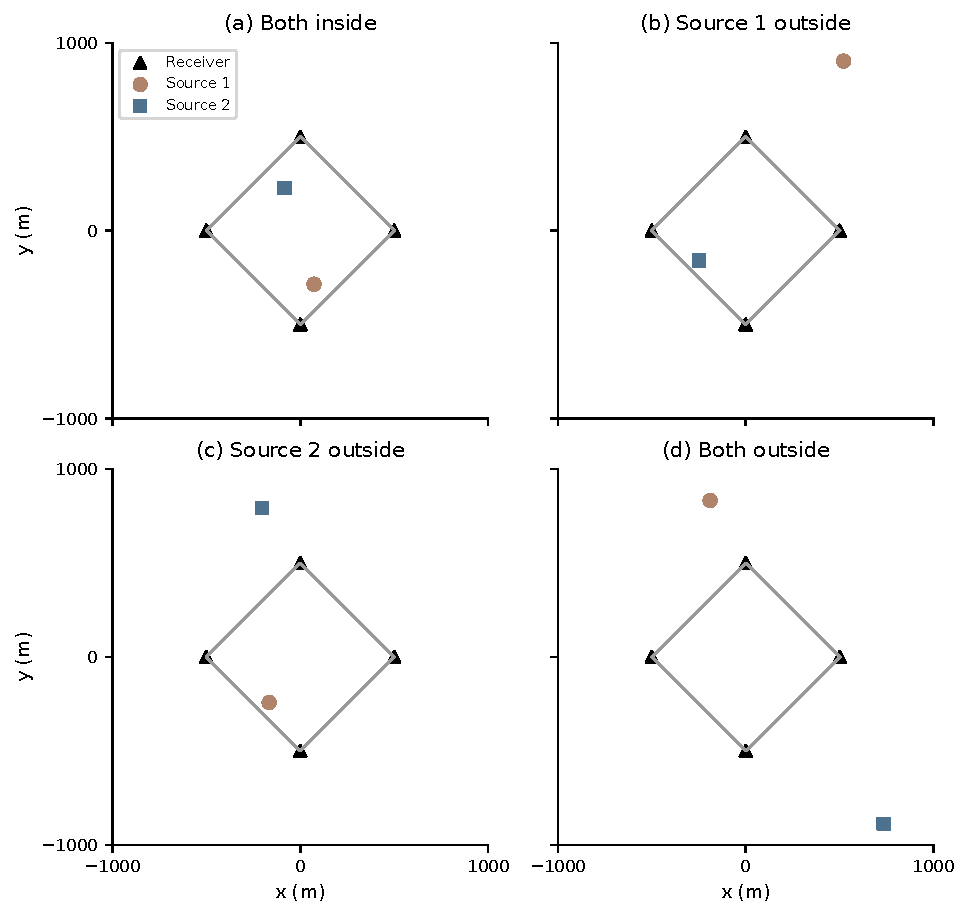
\includegraphics[width=.92\linewidth]{figures/geometry.pdf}
\caption{四类验证布局。三角形为接收站，实线菱形为站点凸包，圆点和方点为源1、源2。四幅图使用相同坐标范围。}\label{fig:geometry}
\end{figure}

\subsection{评价与计时}
设真实位置集合为$X=\{\bm p_k\}$，算法输出的位置集合为$Y=\{\widehat{\bm p}_j\}$。本文预先将容许误差设为最大站间基线的2\%，即$r=0.02R=20$\,m。该门槛用于比较，不由初始网格步长决定。评价时在误差不超过$r$的关联中，先最大化一对一匹配数，再最小化其平方距离和。强源和弱源成功率分别统计源1、源2被匹配的比例；双源成功率要求两源同时被匹配。一个估计位置只能匹配一个真实源。

未截断误差使用独立的最小平方距离指派。等基数情况下
\begin{equation}
 \pi^*=\arg\min_{\pi}\sum_{k=1}^{K}
 \|\bm p_k-\widehat{\bm p}_{\pi(k)}\|_2^2,\qquad
 e_k=\|\bm p_k-\widehat{\bm p}_{\pi^*(k)}\|_2 .\label{eq:assignment}
\end{equation}
其中$\pi$为估计编号的排列，$\pi^*$为总平方距离最小的排列，$e_k$为配对后的第$k$源误差，单位为m。指派用匈牙利算法求解\cite{Kuhn1955}。这种未截断指派与前述门槛匹配分别计算：前者评价全部距离误差，后者统计给定容许误差下的成功次数。对$n_{\mathrm{obs}}$条观测，分别报告
\begin{equation}
 \mathrm{RMSE}_k=\sqrt{\frac1{n_{\mathrm{obs}}}
 \sum_{i=1}^{n_{\mathrm{obs}}}e_{ik}^2},\qquad
 \widehat F_k(t)=\frac1{n_{\mathrm{obs}}}
 \sum_{i=1}^{n_{\mathrm{obs}}}\mathbf 1(e_{ik}\le t),\label{eq:rmseCDF}
\end{equation}
其中$i$为观测编号，$\mathbb 1$为示性函数，$\widehat F_k$为误差经验累计分布（CDF）；P95为误差的第95百分位数。RMSE和CDF使用全部观测，包含超过20\,m的误差，以反映长尾失败。

整体集合误差采用GOSPA\cite{Rahmathullah2017}，$p=2$、$c=100$\,m、$\alpha=2$：
\begin{equation}
 d_{\mathrm G}(X,Y)^2=
 \min_{\gamma}\left[\sum_{(k,j)\in\gamma}\|\bm p_k-\widehat{\bm p}_j\|^2
 +\frac{c^2}{2}\left(|X|+|Y|-2|\gamma|\right)\right],\label{eq:gospa}
\end{equation}
其中$\gamma$为真实与估计位置之间的一对一部分关联，$|X|$、$|Y|$与$|\gamma|$分别为两个集合的基数和关联对数。第一项累计关联距离，第二项按每个未关联位置$c^2/2$计罚；整体距离$d_{\mathrm G}$的单位为m。允许部分关联后，超过$c$的距离可由两个未关联位置的代价替代，从而限制极端误差的影响。20\,m用于判断定位成功，100\,m用于GOSPA代价截断，因此仍需同时报告未截断RMSE。

算法时间从IQ输入后的必要预处理开始，包含DFT、频点筛选、数据传输、搜索、系数求解及精修。GPU运算采用同步计时，公共预热单列。第二组保留求解时间和实验记录开销两个字段，表中使用包含在线轨迹记录的求解墙钟，不含磁盘持久化及事后精度证书。扩大比较将证书成本进一步单列。跨实现比较同时给出运算计数，配对比较则使用相同设备、输入和调用路径。

统计比较保留输入的配对关系。同一波形与噪声实现产生的六档功率差是相关观测，重采样时应一同保留。扩大比较按布局及其内部随机实现分层配对重采样，以给出不确定性区间；四个固定布局的结果则反映这些典型几何下的表现。

\subsection{比较方法及可复现配置}\label{sec:baselines}
所有方法共享公共IQ、传播规律、搜索边界和20\,m初始网格。LS、MUSIC和MVDR在各自谱上选峰并进行相应连续精修；AP、多初值与GA求解式\eqref{eq:profile}；SBL使用多频共享稀疏功率。附录\ref{app:baselines}列出其在本场景下的具体准则。表\ref{tab:parameters}给出当前冻结的扩大比较配置；已完成的较早比较采用的差异在对应结果段说明。
\par\begin{table}[htbp]\centering\footnotesize
\caption{扩大比较的冻结方法参数。连续位置优化不受20\,m网格量化。}\label{tab:parameters}
\begin{tabularx}{\linewidth}{@{}p{.18\linewidth}p{.27\linewidth}X@{}}\toprule
版本 & 核心操作 & 参数\\\midrule
LS谱 & 单源LS谱取两个峰 & 共同20 m网格；同谱连续精修\\
MUSIC & 噪声子空间宽带汇聚 & 4段；超噪声功率加权；已知K\\
MVDR-known & 加载协方差逆谱 & 8段；相对加载0.01\\
充分AP & 反复全域条件更新 & 候选5；循环上限6；正常连续精修\\
交替／联合AP & 相同分支，改变精修方式 & 候选1/2/5；每次局部上限100；共同投影梯度阈值$10^{-8}$\\
VP-BNOMP & 残差发现、消元Newton、共同LS & 循环上限200；每次Newton最多5步；步长上限50 m\\
固定系数BNOMP & 原文对应的固定系数更新 & 循环上限10000；能量阈值$10^{-8}$；局部小步阈值0.01 m\\
多初值联合ML & 同一联合LS目标 & 8个唯一初值：4谱峰+4 Sobol；L-BFGS-B\\
GA联合ML & 同一联合LS目标 & 种群128；最多200代；连续30代停滞停止\\
宽带SBL & 共享功率、离网字典、单点$\gamma$ & 最多300轮；每5轮离网更新；8个活动点；原生停止\\
\bottomrule\end{tabularx}\end{table}
\par
扩大比较登记的运行环境为Windows、Python 3.10.20、NumPy 2.2.6和PyTorch 2.8.0+cu129，GPU为NVIDIA GeForce RTX 4070 Ti SUPER，CPU计算线程设为20。响应与目标使用双精度实数／复数运算。
\par

各方法的频率轴、分段统计、噪声方差和连续精修均按当前观测模型设置，批量响应、缓存与小矩阵求解等计算优化对适用方法共同开放。候选分支和局部更新目标的改变则单独列为算法版本。MUSIC用四个片段估计协方差，按观测功率扣除噪声后的能量进行频率加权；MVDR-known用八个片段，并在协方差对角线上增加平均对角功率的0.01倍。两者处理相同物理频带，具体统计条件与公式见附录\ref{app:baselines}。

\subsection{混合干扰与逐源处理的作用}
图\ref{fig:gap}给出第一组已完成比较。MUSIC与MVDR-known的孤立弱源20条和孤立强源120条均达到20\,m成功门槛，混合后成功率随功率条件变化明显；AP和VP-BNOMP则在该组120条混合观测中全部成功。孤立源对照排除了“弱源本身普遍不可定位”这一主要解释，也说明联合拟合与逐源处理对本场景具有实际作用。
\begin{figure}[htbp]\centering
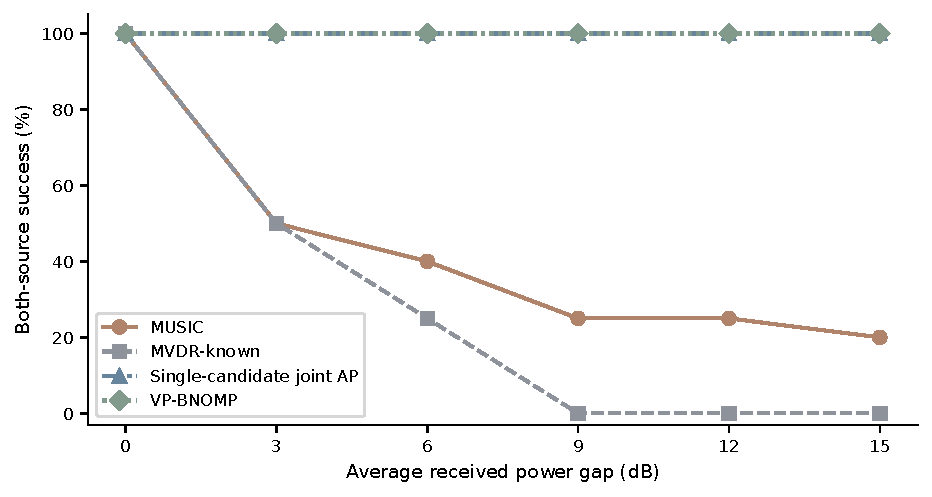
\includegraphics[width=.9\linewidth]{figures/power_gap.pdf}
\caption{公共带限输入下的双源20\,m成功率。每档20条观测，共120条；每个随机实现的六档功率差共享波形与噪声。AP使用单候选联合精修，VP-BNOMP采用波形消元局部更新。}\label{fig:gap}
\end{figure}

这一组比较确立了有竞争力的参照：条件搜索与残差精修能够在本模型下快速处理强弱重叠源。后续实验围绕这些求解器，进一步区分候选恢复和精修成本的收益。

\subsection{候选保留与联合精修的配对结果}\label{sec:apresults}
第二组比较统一初始化与优化精度。单候选交替AP和单候选联合AP均在120条观测中成功110条，位置与最终拟合目标接近；联合精修减少了目标和梯度调用。恢复五候选后，原10条失败全部被正确候选分支恢复。表\ref{tab:paired}给出完整配对结果。
\par\begin{table}[htbp]\centering\small
\caption{相同120条观测的配对结果。RMSE使用全部观测，单位m。}\label{tab:paired}
\begin{tabular}{@{}lrrrrr@{}}\toprule
方法 & 双源成功 & 强源RMSE & 弱源RMSE & GOSPA & 时间/s\\\midrule
单候选交替AP & 110/120 & 0.942 & 103.867 & 10.347 & 0.4071\\
单候选联合AP & 110/120 & 0.942 & 103.866 & 10.347 & 0.3739\\
五候选联合AP & 120/120 & 0.760 & 3.146 & 2.079 & 0.6764\\
VP-BNOMP & 120/120 & 0.761 & 3.146 & 2.078 & 0.5196\\
\bottomrule\end{tabular}\end{table}
\par

\begin{figure}[htbp]\centering
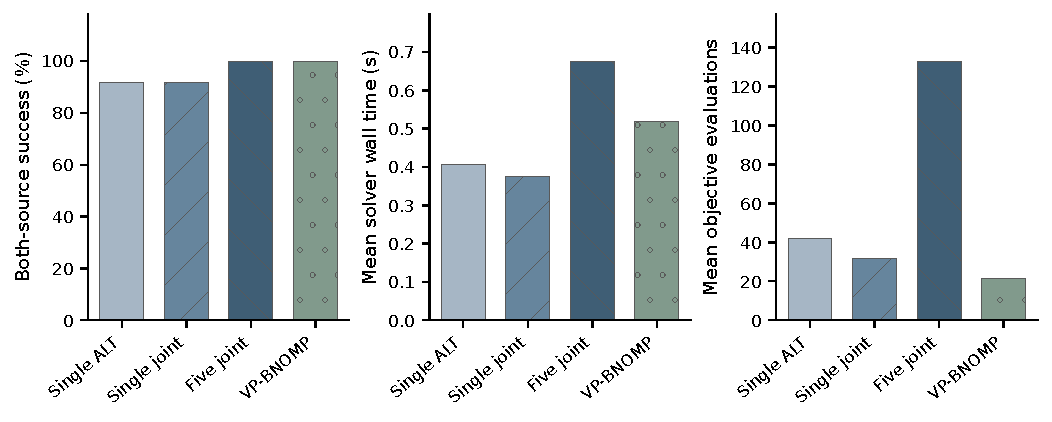
\includegraphics[width=.92\linewidth]{figures/paired_cost.pdf}
\caption{第二组的双源成功率、平均求解墙钟和目标调用次数。前三个AP版本共享输入及共同停止精度；VP-BNOMP保留原生循环停止。五候选成本包括全部分支，不仅统计最终被选分支。}\label{fig:paired}
\end{figure}

单候选联合AP的平均墙钟由0.4071\,s降至0.3739\,s，减少8.15\%；目标调用由41.875次降至31.525次，梯度调用由39.875次降至29.525次。这说明联合精修的主要收益来自计算减少，而非较松的停止条件。五候选联合AP的平均墙钟为0.6764\,s，在增加成本的同时恢复了可靠性。VP-BNOMP平均为0.5196\,s，同样达到120/120成功。两种提出方法在这一组中形成了不同的候选发现和成本取舍。

图\ref{fig:branches}展示多候选发挥作用的一条观测。排名第一的条件候选精修后停留在错误区域，弱源误差为361.21\,m；第二候选精修后误差为0.25\,m，联合残差也更小。两个分支都满足相同精度检验，区别来自进入的局部区域。因而，仅延长第一分支的局部迭代不能替代候选保留。
\begin{figure}[htbp]\centering
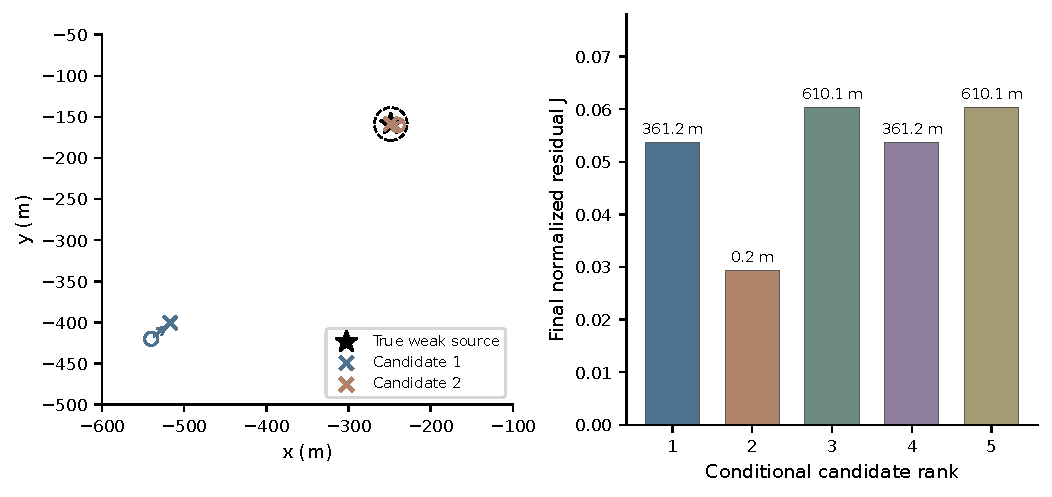
\includegraphics[width=.92\linewidth]{figures/candidate_case.pdf}
\caption{候选恢复案例：源1在站外、源2在站内，功率差6\,dB。左图放大弱源区域，圆圈为候选起点，叉号为精修终点，星号与虚线圆为弱源真值及成功范围；右图使用保存的分支目标与位置误差。该图为事后机制案例，统计结论来自全部120条配对观测。}\label{fig:branches}
\end{figure}

\FloatBarrier
10条恢复观测来自同一个布局中的多个随机实现与功率条件。它们构成候选机制证据；扩大比较将进一步检验这一机制在更多独立几何中的出现频率。图\ref{fig:cdf}保留全部误差，展示成功率之外的长尾变化。
\begin{figure}[htbp]\centering
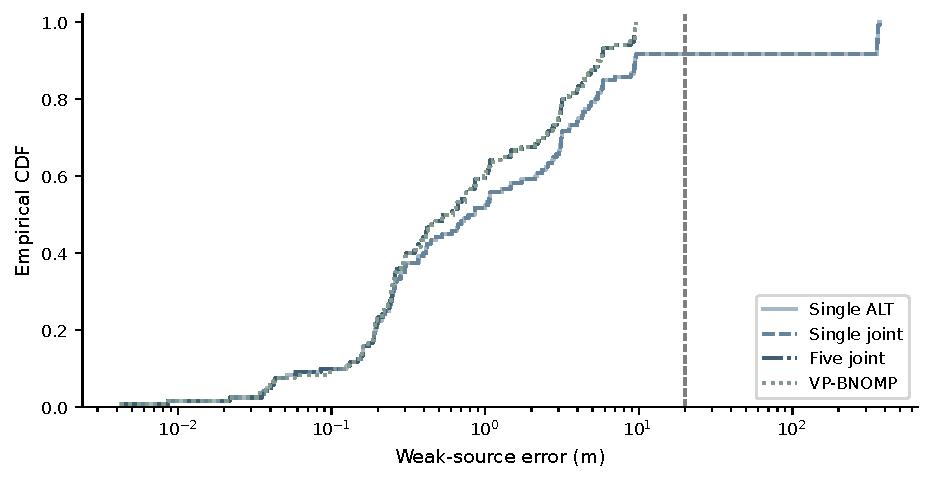
\includegraphics[width=.9\linewidth]{figures/error_cdf.pdf}
\caption{第二组弱源误差CDF，包含全部120条观测；虚线标出20\,m成功门槛。对数横轴展示亚米误差与数百米长尾。}\label{fig:cdf}
\end{figure}

\subsection{固定系数与消元曲率的机制实验}\label{sec:mechanismresults}
为区分停止尺度、数值保护和局部目标的影响，第三组在四个布局、0/15\,dB两档的八条观测上作受控比较。固定系数参照使用原文对应的局部Newton形式、共同系数重估时序和能量停止；消元对照只替换局部位置目标，保留其余时序。另比较放宽能量停止阈值以及取消局部小步长退出，结果见表\ref{tab:mechanism}。
\par\begin{table}[htbp]\centering\small
\caption{八条观测的曲率机制隔离。各行共享相同输入和外层系数更新时序。}\label{tab:mechanism}
\begin{tabular}{@{}lrrrr@{}}\toprule
局部更新与停止 & 双源成功 & 弱源RMSE/m & 时间/s & 导数调用\\\midrule
固定系数，严格停止 & 8/8 & 5.413 & 5.4783 & 2679.500\\
固定系数，阈值$10^{-7}$ & 7/8 & 9.665 & 2.3184 & 1133.875\\
固定系数，阈值$10^{-6}$ & 6/8 & 12.683 & 0.9706 & 467.375\\
固定系数，取消小步退出 & 8/8 & 2.011 & 8.0110 & 4758.375\\
消元更新，严格停止 & 8/8 & 3.221 & 0.4356 & 70.375\\
\bottomrule\end{tabular}\end{table}
\par

\begin{figure}[htbp]\centering
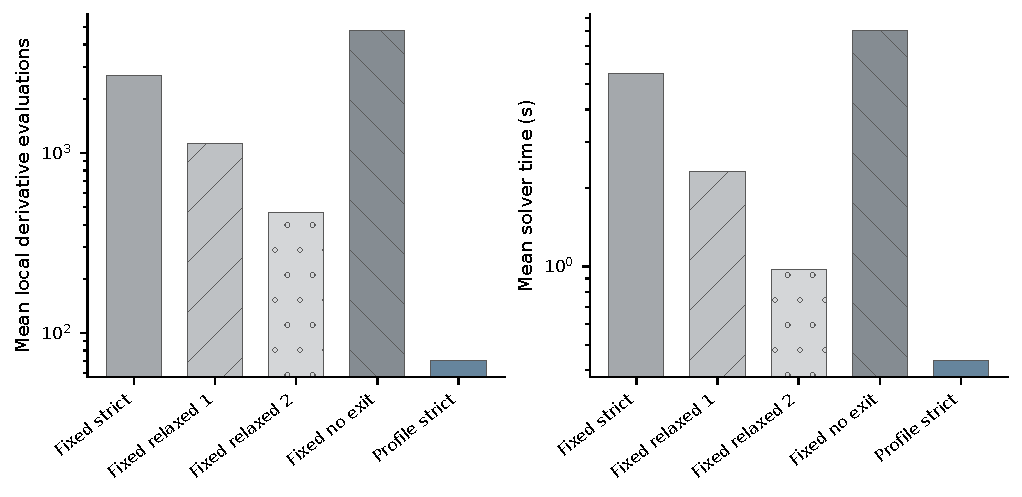
\includegraphics[width=.9\linewidth]{figures/curvature_cost.pdf}
\caption{八条观测的受控曲率实验。左为平均局部导数调用数，右为平均求解时间；纵轴为对数刻度。严格固定系数与严格消元更新共享停止尺度及外层时序。}\label{fig:curvature}
\end{figure}

严格固定系数更新的21436次局部步中，有17935次以已接受的小步触发局部退出，占83.7\%。这些步已使局部目标下降，但位置移动很小，外层循环仍需再次进入局部精修。这组运行未触发Hessian修正、步长截断、边界裁剪或回溯，记录支持将主要计算损失归于反复的小步更新。将目标下降阈值从$10^{-8}$放宽至$10^{-7}$或$10^{-6}$虽然省时，却降低了20\,m成功数。取消小步退出则增加了计算。

保持严格阈值后，消元更新的平均导数调用从2679.5次降至70.375次，平均时间从5.4783\,s降至0.4356\,s，两者均保持8/8成功。这与式\eqref{eq:schur}所揭示的位置--系数耦合机制一致。该倍率对应八条观测的隔离对照，不作为整套VP-BNOMP在扩大数据上的最终加速比。

\subsection{扩大布局的统一比较}\label{sec:formalpending}
扩大比较已冻结20个布局，四类内外关系各五个布局，每布局20次波形与噪声实现，六档功率差，共2400条混合观测。六个核心版本共享全部2400条输入；八类方法及原文对应BNOMP在共同240条子集上比较，慢方法独立完成后补入同一报告。各阶段保留早期解、最终解、原生停止与实际运算计数。

核心版本包括VP-BNOMP及其末端联合变体、单候选交替AP，以及候选数为1、2、5的联合AP。采用嵌套候选和共同前缀，避免把不同初始化或停止尺度混入部件收益。20个布局中，各类别的前3个用于分析，后2个为锁定验证。正式报告将分别给出分功率差成功率、误差、完整耗时和调用次数，并以布局与随机实现的层次配对统计反映不确定性。

\pending{扩大比较正在运行。本节只登记已经冻结的设置；正式成功率、误差、耗时、区间及方法排名待逐样本审计完成后填入，并据此定稿摘要和结论。}
